\part{Gouvernements et Organisation}

\begin{center}
	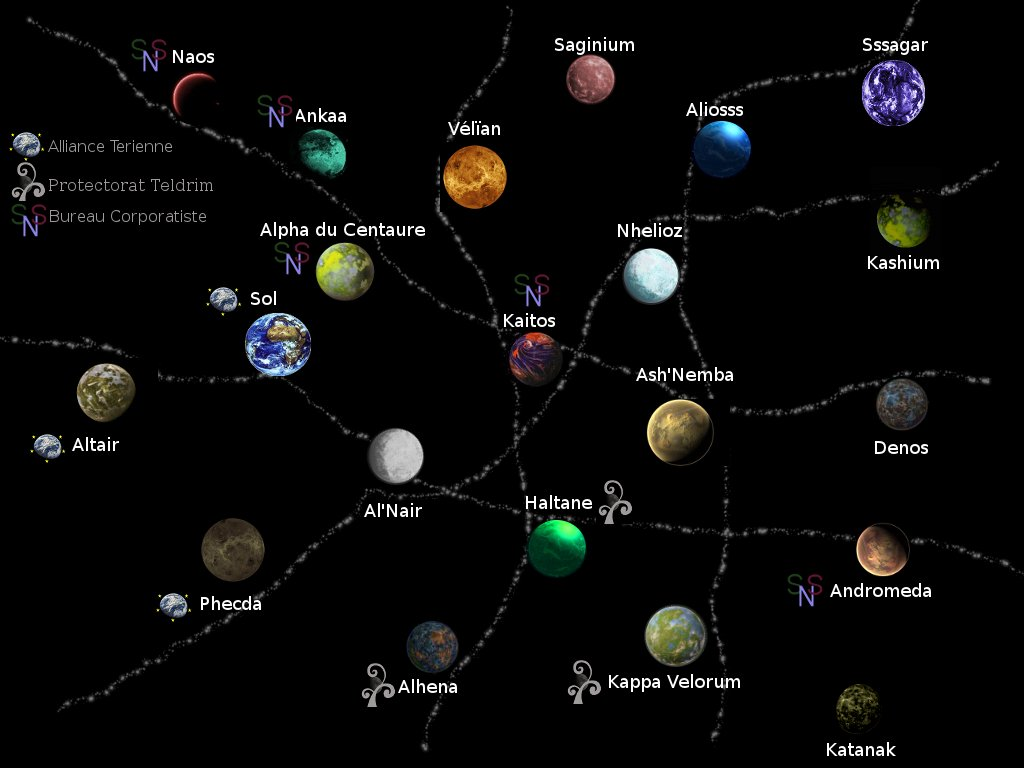
\includegraphics[scale=0.45]{Img/new_carte}
\end{center}

\chapter{Gouvernements}

\begin{multicols}{2}

\section{Alliance Kaitéenne}

Au tout début de la seconde guerre, l'Alliance Kaitéenne était le gouvernement le plus puissant. Tous craignaient son hégémonie, d'autant plus que l'Alliance avait un but expansionniste avoué : elle voulait créer un gouvernement unique couvrant l'ensemble des mondes connus. Elle voulait créer un empire interstellaire capable de résister à d'autres peuples (Vélïos, Eskadors, Ergios) s'ils osaient revenir.

La naissance du Bureau Corporatiste fut pour l'alliance Kaitéenne une épine dont elle ne s'est pas remise. Aujourd'hui l'alliance, privée de son centre névralgique et d'une partie de ses têtes pensantes, essaie tant bien que mal de se restructurer. Heureusement pour elle, le Bureau Corporatiste est maintenant occupé sur d'autres fronts, leur laissant l'occasion de reprendre leur souffle.


\subsection{Ce que sa population pense de...}

\begin{itemize}
\item Protectorat Teldrim : Ce pourrait être des alliés sérieux, nous allons tout faire pour les convaincre.
\item Alliance des Nations Terriennes : Nous comptions sur eux mais ils nous ont trahis. Nous espérons qu'ils vont perdre la guerre face aux Teldrims.
\item Consortium Technologique : Ces lézards moralisateurs doivent faire face à une prise de pouvoir chez eux ! Quelle ironie ! Malheureusement nous craignons que le Consortium ne soutienne le bureau.
\item Bureau Corporatiste : Ces chiens nous ont pris par surprise mais nous ne somme pas encore vaincus. Nous les réduirons à néant.
\item Conseil Nomade : Nous les tolérons uniquement car ils sont totalement négligeables.
\item Empire Vélïos : Les Vélïos se rendront vite compte de la félonie des corporations et nous rejoindrons alors dans la lutte.
\end{itemize}

\section{Protectorat Teldrim}

\begin{center}

\includegraphics[scale=0.2]{Img/logo_teld}
\end{center}

Le Protectorat Teldrim est la zone d'influence issue de la planète mère des Teldrims, Kappa Velorum. Il s'agit d'une alliance entre les grandes espèces Teldrims menée par la prêtrise. Les prêtres sont les porteurs de l'autorité de l'Eglise et y ont tous les droits. Être prêtre dans le Protectorat Teldrim est un peu comme être un noble sur son territoire à l'ère médiévale.

Sur Kappa Velorum et Haltane, seuls les Teldrims (n'appartenant pas à la race des esclaves, évidemment) ont le statut de citoyen. Les autres peuples sont, au mieux, des Paria qu'on tolère tant qu'ils ne créent pas de problème. Sur Alhena, la situation s'est un peu allégée, et seuls les Teldrims de la race esclave sont réellement perçus comme inférieurs. Le système étant peuplé à plus de 50\% par des non-Teldrims, les prêtres ont bien été obligés de s'adapter.

\begin{itemize}
\item Alliance Kaitienne : Nous avions tous des envies de conquêtes mais l'alliance a eu le courage d'assumer les siennes. Ça leur à toutefois couter cher, dommage...
\item Alliance des Nations Terriennes : Nous n'avons rien de personnel contre eux. Ils ont été trop gourmand et ont juste rencontrés plus puissant qu'eux.
\item Consortium Technologique : Nous estimons les Snagirs pour leurs savoir. Nous comptons sur leur aide quand il nous faudra affronter le Bureau.
\item Bureau Corporatiste : Ils veulent régner sur les mondes connus. Pour l'instant ils sont occupés avec l'alliance mais il nous faudra un jour les affronter.
\item Conseil Nomade : Qu'importe les nomades ! Qu'ils continuent à vivre isoler, ils ne nous intéressent pas.
\item Empire Vélïos : Seul l'avenir nous dira si nous pouvons faire confiance ou non à l'impératrice.
\end{itemize}

\section{Alliance des Nations Terriennes}

\begin{center}

\includegraphics[scale=0.3]{Img/logo_at}
\end{center}

Aujourd'hui encore, la Terre est partagée entre différentes nations qui se livrent une guerre tantôt militaire, tantôt économique. Mais, devant la menace constituée par les autres gouvernements de la Deneb, les nations terriennes se sont enfin décidées à se réunir sous l'égide d'une alliance solide. L'unité n'est pas encore faite, mais les terriens ont appris à faire front commun vis à vis des autres nations interstellaires.

\subsection{Ce que sa population pense de...}

\begin{itemize}
\item Alliance Kaitienne : Des opportunistes qui n'ont que ceux qu'ils méritent. Mais espérons toutefois qu'il donne encore un peu de fil à retordre aux corporations.
\item Protectorat Teldrim : Ces bêtes ont réussit à prendre l'avantage à cause de leurs nombres, mais notre supériorité est flagrante et nous allons bientôt leur faire connaître.
\item Consortium Technologique : L'ancien gouvernement Snagir était mou et totalement inutile. Voyons voir ce que nous réserve celui-ci.
\item Bureau Corporatiste : Les corporations devraient savoir se tenir à leur place et s'occuper uniquement de faire du profit. La population découvrira bientôt qu'il leur faut des vrai dirigeants.
\item Conseil Nomade : Autrefois nous les avons négligés, mais nous avons apprit de nos erreurs. Les nomades pourraient peut-être faire de bon amis.
\item Empire Vélïos : L'impératrice n'est pas une allié fiable, nous en savons quelque chose. Elle prépare surement une traitrise mais nous somme prêt.
\end{itemize}

\section{Consortium Technologique}

Le Consortium Technologique est, depuis des siècles, la corporation la plus importante du peuple Snagir. Certains financiers disent qu'il s'agit même de la seule corporation. Il faut avouer qu'en cherchant un peu, on se rend compte que toutes les corporations Snagirs appartiennent de près ou de loin au consortium.

Jusqu'à maintenant, le gouvernement Snagir était un organe pyramidal extrêmement lent. La moindre décision nécessitait de multiples votes. Devant la réactivité nécessaire pour faire face à la seconde guerre, le Consortium décida de faire un coup d'état et de prendre les commandes. Le plus étonnant dans tout ça est que le Consortium a réussi sa prise de pouvoir sans effusion de sang, éveillant à peine quelques protestations. Les analyses tendent à démontrer que le Consortium préparait son coup depuis de très longs siècles, mais la chose reste à prouver.

Depuis, les Snagirs affichent une stratégie plus agressive. Militairement, ils se contentent toujours de protéger leurs frontières. économiquement, ils livrent une guerre sans merci aux autres nations ce qui crée de multiples tentions, notamment avec le Bureau Corporatiste. Récemment, il paraîtrait que leurs forces ont commencé à s'activer de plus en plus dans la guerre "de l'ombre" (sabotage, espionnage, manipulation ...)

\subsection{Ce que sa population pense de...}

\begin{itemize}
\item Alliance Kaitienne : Nous soutenons le bureau dans la guerre contre l'alliance. Le tyran qui est à sa tête doit tomber.
\item Protectorat Teldrim : Ils ont gagnés la guerre mais doivent maintenant s'arrêter et laisser la nation terrienne panser ses plaies. Nos diplomates œuvre en ce sens.
\item Alliance des Nations Terriennes : Il est temps que l'alliance cède sa place à un gouvernement capable d'unir réellement les peuples humains.
\item Bureau Corporatiste : Les corporations ont fait une bonne chose en arrêtant l'alliance, mais elles ne s'arrêteront pas là. Quand le moment sera venu nous seront là pour l'arrêter.
\item Conseil Nomade : Inutile de s'occuper d'eux, ils ne font aucun mal là où ils sont.
\item Empire Vélïos : L'impératrice est sage, elle a donc un plan derrière la tête, mais lequel ? Dur à savoir...
\end{itemize}

\section{Bureau Corporatiste}

\begin{center}

\includegraphics[scale=0.2]{Img/logo_corpo}
\end{center}

Au début de la seconde grande guerre, les grandes Corporations ont menacé les gouvernements, leur annonçant qu'elles n'accepteraient pas la présence de blocus. Le marché devait rester libre ou elles forceraient le passage militairement. Leur menace a été prise à la légère et très vite, des flottes de blocus se mirent en place. Quelle ne fut pas la surprise du monde connu quand on apprit, un jour, qu'une flotte de l'Alliance Kaitéenne avait été mise en défaite par une flotte d'origine Corporatiste.

Les gouvernements avaient oublié que certaines corporations étaient déjà bien armées (SML) et que, possédant une grande partie de l'industrie, les corporations n'auraient aucun mal à renforcer leurs flottes. Une nouvelle force venait de voir le jour.

Une fois les hostilités engagées, il ne fallut pas longtemps à certaines grandes corporations comme la SML, Senstech, et la Guilde Nova pour changer de politique et commencer à créer un Protectorat, créant ainsi le Bureau Corporatiste.

Très vite, le Bureau Corporatiste devint le pire ennemi de l'Alliance Kaitéenne et de son ambition expansionniste. Certaines planètes décidèrent de se placer d'elles-même sous la protection des corporations. C'est le cas, par exemple, d'Alpha Centauri.

\subsection{Ce que sa population pense de...}

\begin{itemize}
\item Alliance Kaitienne : La soif de pouvoir de l'alliance nous a forcé à devenir un véritable gouvernement. Nous pouvons les remercier pour cela mais l'alliance doit disparaitre.
\item Protectorat Teldrim : Ils deviennent trop puissants, il nous faudra les arrêter comme nous avons stoppé l'alliance. 
\item Alliance des Nations Terriennes : Ils comprendront bientôt que leur intérêt est de nous rejoindre, en attendant laissons les se débrouiller avec les Teldrims.
\item Consortium Technologique : Nous savons pas encore quoi penser d'eux. Nos contacts diplomatiques sont bons mais cela va-t-il durer ?
\item Conseil Nomade : Nous comptons en faire des alliés. Ils sont présents dans tous les mondes connus et pourrait nous fournir de nombreux renseignements.
\item Empire Vélïos : L'impératrice a eu la sagesse de rentrer en contact avec nous, sa puissance nous serait très utile.
\end{itemize}

\section{Conseil Nomade}

\parpic[r]{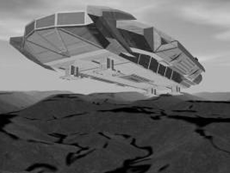
\includegraphics[width=120pt]{image/vaisseau4.png}}Autrefois, les Nomades vivaient dans des clans disparates, n'entretenant que des contacts irréguliers entre eux. Les groupuscules étaient éloignés philosophiquement, financièrement, économiquement, et les modes de gouvernance différaient. 

Puis, des gouvernements voulurent les forcer à se plier à leurs règles, à leurs manières de voir les choses. Ils voulurent les soumettre. Ils demandèrent aux nomades de participer à l'effort de guerre. Ce fut une grave erreur. 
 
Au début, les Nomades se soumirent. Mais en réalité, ils commencèrent à reprendre contact avec les stations les plus proches. Un réseau commença à se créer. Les nomades s'organisèrent alors pour reprendre leur liberté. L'opération fut mûrement réfléchie et les préparatifs effectués sur de longues années. Les jeunes nomades furent envoyés rejoindre l'effort de guerre en plus grand nombre. Les gouvernements ne se doutèrent de rien.

Puis, un jour, les Nomades déclarèrent à nouveau leur indépendance. Voulant riposter, les gouvernements leur ayant forcé la main découvrirent que certains vaisseaux militaires avaient été détournés. Ces vaisseaux constituaient alors la nouvelle force de défense Nomade. Le gouvernement Nomade était né, composé d'un grand conseil réunissant un représentant de chaque clan.

Depuis, l'union s'est renforcée. Au gré des alliances, au gré des mariages, le nombre de clans s'est réduit pour laisser place à des clans plus puissants. Pour l'instant, le conseil s'occupe uniquement de sauvegarder l'indépendance Nomade. Mais il représente maintenant une force non négligeable dont tout le monde se méfie. Les nomades pourraient bien choisir un jour un camp, et nul ne sait lequel ce sera.

\subsection{Ce que sa population pense de...}

\begin{itemize}
\item Alliance Kaitienne : Ce sont des nuisibles qui méritent de disparaitre.
\item Protectorat Teldrim : Le protectorat prône l'esclavage et le jour où ils domineront les mondes connus il l'imposeront à tous. Rien que pour cette raison nous pensons qu'il faut lutter contre eux.
\item Alliance des Nations Terriennes : Ils perdent la guerre contre les Teldrims. S’ils nous négligeaient un peu moins nous serrions prêt à leur prêter assistance.
\item Consortium Technologique : Ils sont censés et nous laissent vivre en paix. Toutefois ils sont un peu xénophobe et nous nous méfions d'eux pour cela.
\item Bureau Corporatiste : Nous avons de très bon contact avec les corporatistes. Une alliance est d'ailleurs en discussion avec eux.
\item Empire Vélïos : Les Vélïos Fédéraux semblent se méfier de l'impératrice, malheureusement le bureau n'écoute pas nos avertissements.
\end{itemize}

\section{Empire Vélïos}

Autrefois les Vélïos avaient rejoint la Fédération comme les autres races. Ils ne possédaient alors qu'un seul système solaire : Vélians. Durant la première guerre galactique, les Vélïos se sont repliés sur eux-même et ont fermé leurs frontières, sans explication. Après le départ des Ergios, ils n'ont pas voulu rompre leur isolement. Puis, quand la capitale a subi l'assaut de ces extraterrestres inconnus, les Eskadors, les Vélïos sont venus au secours de la Fédération. Pourquoi ? Comment ont-ils su ?

Aujourd'hui les analystes pensent que les Vélïos était entrés en conflit avec les Eskadors bien avant le reste des mondes connus. Quand ? Les Vélïos n'ont pas voulu non plus répondre à cette question. Toutefois s'ils sont affrontés ces extraterrestes avant nous, ils ont sûrement découvert le moyen de voyager sans les portails bien avant nous également. Combien de monde les Vélïos ont-ils conquis aujourd'hui ? C'est une des autres questions auxquelles ils ne répondent pas...

\subsection{Ce que sa population pense de...}

Les territoires Vélïos restent fermés et nul ne sait ce que pense sa population.

\end{multicols}
